\subsection{Reprezentacja danych}
Reprezetancja za pomoca wektora binarnego gdzie jedynke interpretujemy jako kondydature oferty do zaakceptowania, a zero za brak oferty w zbiorze ofert zaakceptowanych.
Jeżeli oferta posiada jedynke w wektorze czyli jest kandydatem do zaakceptowania nie oznacza jeszcze, że zostanie dodana do zbioru ofert zaakceptowanych.

Dzięki takiej reprezentacji możemy zastosować algorytm PBIL do rozwiązania tego problemu.

\subsection{Funkcja celu}
Oferty oznaczone jedynka rozumiemy jako oferty zaakceptowany. Dopuszczamy jednak możiwość występownia dwóch ofert zaakceptowanych o nierozłoącznym zbiorze towarów, ale wtedy preferujemy tą o mniejszym indeksie

\subsection{Rozwiązanie}
Do rozwiązania tego problemu użyliśmy algorymu PBIL.
Współczyniki uczenia, prawdopodobieństwa mutacji i zaburzenia podczas mutacji ustawiliśmy kolejno na 0.2, $\frac{1}{\text{liczba ofert}}$ i 0.1.
Liczbe iteracji ustawialiśmy na 100, a populacje na 20.

\subsection{Wyniki}
Wyniki zaprezentowane są na wykresach poniżej (\ref{wyk:pbil1}, \ref{wyk:pbil2}).
Niebieską linią oznaczyliśmy najepszego osobnika dla algorytmu PBIL w danej iteracji. Zieloną najlepszy wynik algorytm losowego, który wybierał z takiej samej puli losowych osobników ile łącznie przegląda PBIL.
\begin{figure}[!ht]
    \centering
    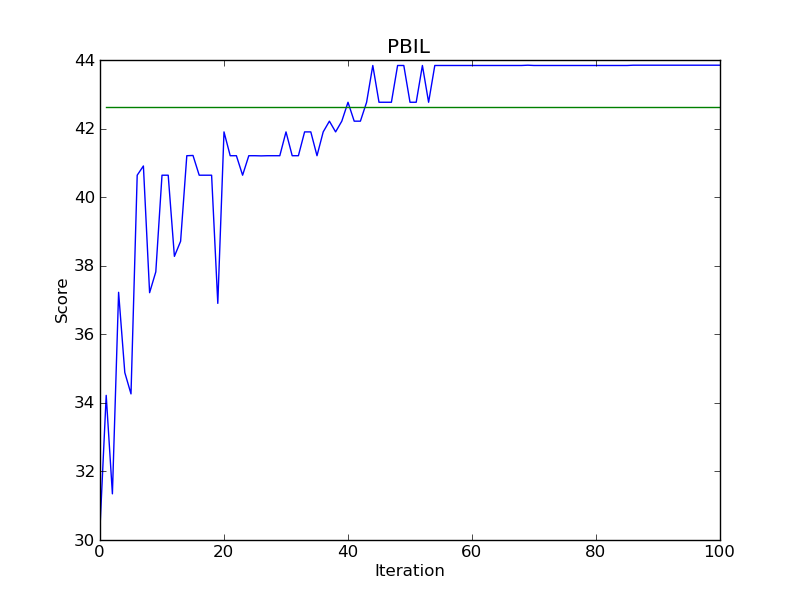
\includegraphics[width=10cm]{wykresy/matching_bids_100_goods_20_0000_txt_pbil.png}
    \caption{Wykres dla problemu 'matching' z 20 ofertami i 100 towarami.}
    \label{wyk:pbil1}
\end{figure}

\begin{figure}[!ht]
    \centering
    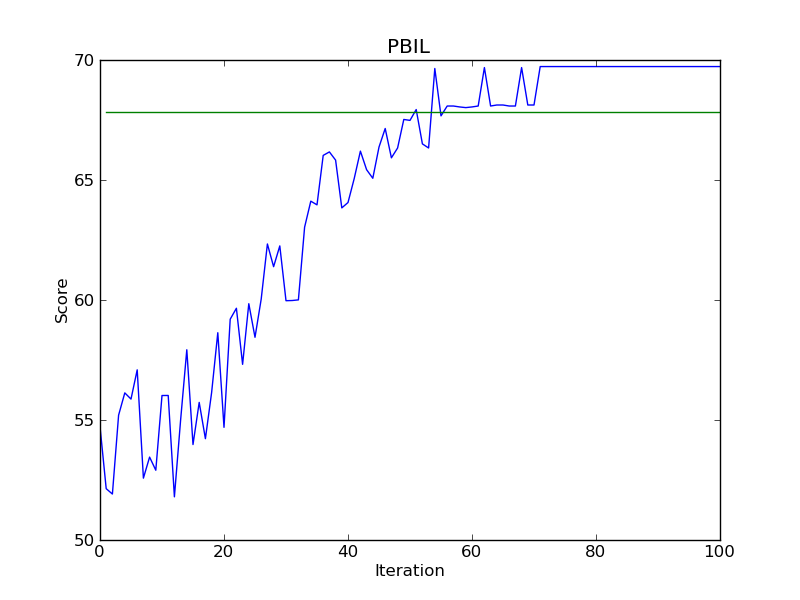
\includegraphics[width=10cm]{wykresy/matching_bids_100_goods_40_0000_txt_pbil.png}
    \caption{Wykres dla problemu 'matching' z 40 ofertami i 100 towarmi.}
    \label{wyk:pbil2}
\end{figure}
